\documentclass[10pt]{article}

% Defining page margins
\usepackage[top=1in, bottom=1.5in, left=1in, right=1in]{geometry}
% Ability to generate urls
\usepackage{hyperref}
% Ability to display pseudocode
\usepackage{algorithm}
\usepackage[noend]{algpseudocode}
% Nice graphs
\usepackage{tikz}
% Nice arrows for directed graphs
\usetikzlibrary{arrows.meta,arrows}
% Define colors + coloring cells o tables
\usepackage{color, colortbl}
% Text over right arrow (see: http://tex.stackexchange.com/questions/103988/rightarrow-with-text-above-it)
\usepackage{mathtools}

% Ability to create cells with few lines of text
% see: http://tex.stackexchange.com/questions/2441/how-to-add-a-forced-line-break-inside-a-table-cell
\newcommand{\specialcell}[2][c]{%
  \begin{tabular}[#1]{@{}l@{}}#2\end{tabular}}
  
% Align comment in the same way as Stetements in pseudocode
% see: http://tex.stackexchange.com/questions/74880/algorithmicx-package-comments-on-a-single-line
\algnewcommand{\LineComment}[1]{\State \indent \(\triangleright\) #1}
  
\definecolor{Gray}{gray}{0.9}

\begin{document}

\title{Inference of chemical compound types \\ using graph of chemical reactions}
\author{Yurii Lahodiuk \\ yura.lagodiuk@gmail.com}
\date{}
\maketitle

\begin{abstract}
% TODO: refactor
In this article we will consider representation of information about chemical reactions - from the point of view of graph theory. We will expose some properties of chemical reactions graph in order to infer types of chemical compounds, and do this in polynomial time. And, finally, I would like to provide detailed description of developed programming framework\cite{project_on_github} for approximate inference over pairwise Markov Random Fields, with appliance to such examples as: decoding of Low-density parity-check codes, Coloring of graph, Fraud detection using network effects\cite{fraud_detection}.
\end{abstract}

\section{Problem statement}
Lets imagine simplified universe, where exists only few different \emph{types of chemical compounds}. 
Also there exists restrictions on \lq \lq allowed\rq \rq\ interactions between different kinds of compounds (lets call these restrictions -- \emph{types of chemical reactions}). For example:

\begin{table}[!htb]
    \begin{minipage}{.2\linewidth}
      \centering
        \begin{tabular}{| l |}
            \hline
            \rowcolor{Gray}
            \specialcell{Compound \\ Type} \\ \hline
            $Water$ \\ \hline
            $Base$ \\ \hline
            $Acid$ \\ \hline
            $Salt$ \\ \hline
            $Acidic\ Salt$ \\ \hline
            $Acidic\ Oxide$ \\ \hline
            $Basic\ Oxide$ \\ \hline
        \end{tabular}
    \end{minipage}%
    \begin{minipage}{.8\linewidth}
      \centering
        \begin{tabular}{| l | l |}
            \hline
            \rowcolor{Gray}
            Reaction Type & Example \\ \hline
            $Base + Acid \rightarrow Salt + Water$ & $2NaOH + H_{2}SO_{4} \rightarrow Na_{2}SO_{4} + 2H_{2}O$ \\ \hline
            $Base + Acid \rightarrow Acidic\ Salt + Water$ & $NaOH + H_{2}SO_{4} \rightarrow NaHSO_{4} + H_{2}O$ \\ \hline
            $Acidic\ Salt + Base \rightarrow Salt + Water$ & $NaHSO_{4} + NaOH \rightarrow Na_{2}SO_{4} + H_{2}O$ \\ \hline
            $Basic\ Oxide + Water \rightarrow Base$ & $Na_{2}O + H_{2}O \rightarrow 2NaOH$ \\ \hline
            $Acidic\ Oxide + Water \rightarrow Acid$ & $SO_3 + H_{2}O \rightarrow H_{2}SO_4$ \\ \hline
            $Acidic\ Oxide + Base \rightarrow Salt + Water$ & $SO_3 + 2NaOH \xrightarrow{t} Na_{2}SO_4 + H_{2}O$ \\ \hline            
            $Salt + Water \rightarrow Base + Acid$ & \specialcell{$Al_{2}(SO_{4})_3 + 6H_{2}O \xrightarrow{t}$ \\ \hspace{5em}$2Al(OH)_3 \downarrow + 3H_{2}SO_4$} \\ \hline            
        \end{tabular}
    \end{minipage} 
\end{table}

So, this is the only prior knowledge about our simplified universe\footnote{Of course, from the point of view of Chemistry Science - provided model of universe is very rough and strict. But, on the other hand - our model is pretty generic, because it does not depend on details of internal structure of compounds, or any other physical-chemistry factors: \emph{all prior knowledge we have - is just possible types of compounds, and axioms about allowed types of interaction}.}.\\

Now, imagine that we observed reactions of exact chemical compounds.
% TODO: enumerate examples of observed chemical reactions.
% E.g.: NaOH + H2SO4 --> Na2SO4 + H2O, Na2O + SO3 --> Na2SO4, etc.
So, the problem is: \textsl{having described prior knowledge about types of chemical compounds and restrictions on possible types of interactions - needed to \textbf{infer types of compounds, which participate in observed reactions}}. \\

In other words, we can formulate our problem - as \textsl{\textbf{finding of such configuration of types of compounds} from observed reactions, \textbf{which does not violate restrictions on allowed types of interaction}}.

\newpage

\section{Na\"{\i}ve approach}
The most straightforward approach for solving of described problem -- would be just \emph{brute-force search} of appropriate types for chemical compounds from observed reactions:

\begin{algorithm}
\caption{Brute-force search for appropriate types of compounds}\label{alg:brute_force}
\begin{algorithmic}[1]

\State \textbf{explanation of variables:}
\LineComment{\emph{PossibleCompoundTypes} - Array of possible types of compounds}
\LineComment{e.g.: [$Water$, $Base$, $Salt$, $Acid$, $\ldots$]}
\\
\LineComment{\emph{PossibleEquationTypes} -- Set of possible types of reactions}
\LineComment{e.g.: \{\lq \lq$Water + Basic\ Oxode \rightarrow Base$\rq \rq , \lq \lq$Acid + Base \rightarrow Salt + Water$\rq \rq, $\ldots$\}}
\\
\LineComment{\emph{ObservedEquations} -- Array of observed reactions}
\LineComment{e.g.: [\lq \lq$NaOH + H_{2}SO_4 \rightarrow H_{2}O + Na_{2}SO_4$\rq \rq, $\ldots$]}
\\
\LineComment{\emph{compoundsList} -- List of compounds (from observed reactions)}
\LineComment{e.g.: [$H_{2}O$, $NaOH$, $H_{2}SO_4$, $Na_{2}SO_4$, $\ldots$]}
\\
\LineComment{\emph{compoundTypeMap} -- Map with hypothesis about types of compounds (from observed reactions)}
\LineComment{e.g.: \{$H_{2}O \Rightarrow Water$, $NaOH \Rightarrow Base$, $\ldots$\}}
\\
\Procedure{AssignTypes}{$compoundTypeMap, compoundsList$}
    \If{\Call{Empty}{$compoundsList$}}
        \If{\Call{SolutionAcceptable}{$compoundTypeMap$}}
            \State \textbf{return $compoundTypeMap$}
        \EndIf
    \Else
        \State $compound \gets \Call{Head}{compoundsList}$
        \State $restCompounds \gets \Call{Tail}{compoundsList}$
        \For{$i \gets [1..\Call{Size}{PossibleCompoundTypes}]$}
            \State $type \gets PossibleCompoundTypes[i]$
            \State $compoundTypeMap[compound] \gets type$
            \State \Call{AssignTypes}{$compoundTypeMap,restCompounds$}
        \EndFor
    \EndIf
    %TODO: consider, whether it is fine to return such message
    \State \textbf{return} \lq \lq Solution Does Not Exist\rq \rq
\EndProcedure
\\
\Procedure{SolutionAcceptable}{$compoundTypeMap$}
    \For{$i \gets [1..\Call{Size}{ObservedEquations}]$}
        \State $equation \gets ObservedEquations[i]$
        \State $subst \gets \Call{SubstituteTypes}{equation, compoundTypeMap}$
        \LineComment{e.g.: substituting \lq \lq $NaOH + H_{2}SO_4 \rightarrow H_{2}O + Na_{2}SO_4$\rq \rq}
         \LineComment{to \lq \lq $Acid + Base \rightarrow Salt + Water$\rq \rq}
        \If{$\Call{NotContains}{PossibleEquationTypes, subst}$}
            \State \textbf{return $false$}
        \EndIf
    \EndFor
    \State \textbf{return $true$}
\EndProcedure
\end{algorithmic}
\end{algorithm}

The problem of given approach, is such, that it leads to exponential complexity, with growth of number of observed compounds.

\newpage

\section{Chemical reactions as a graph}

Lets represent observed chemical reactions as a graph: 
\begin{itemize}
    \setlength \itemsep{0em}
    \item Each unique chemical compound will be represented as \emph{compound node}
    \item Each observed reaction will be represented as \emph{reaction node}
    \item In case, if chemical compound participates in reaction -- we will connect corresponding \emph{compound node} with corresponding \emph{reaction node}. This means, that graph will not contain edges between nodes of the same type\footnote{Based on this condition we can conclude, that constructed graph is actually \emph{bipartite graph}}
    \item Direction of edge -- reflects role of chemical compound in reaction (\textbf{for reagents}: \emph{direction from compound node -- to reaction node}, and \textbf{for products}: \emph{direction from reaction node -- to compound node})
\end{itemize}

\noindent For example, lets consider subset of three observed reactions\footnote{Reactions displayed without balancing coefficients, because for our purpose, coefficients does nor matter}:

\begin{enumerate}
    \setlength \itemsep{0em}
    \item $NaOH + H_{2}SO_{4} \rightarrow Na_{2}SO_{4} + H_{2}O$
    \item $NaOH + SO_{3} \rightarrow Na_{2}SO_{4} + H_{2}O$
    \item $Na_{2}O + H_{2}O \rightarrow NaOH$
\end{enumerate}

\noindent For these reactions we can construct following graph:


% Might be helpful for the further refactoring: http://www.texample.net/tikz/examples/feature/nodes-and-shapes/
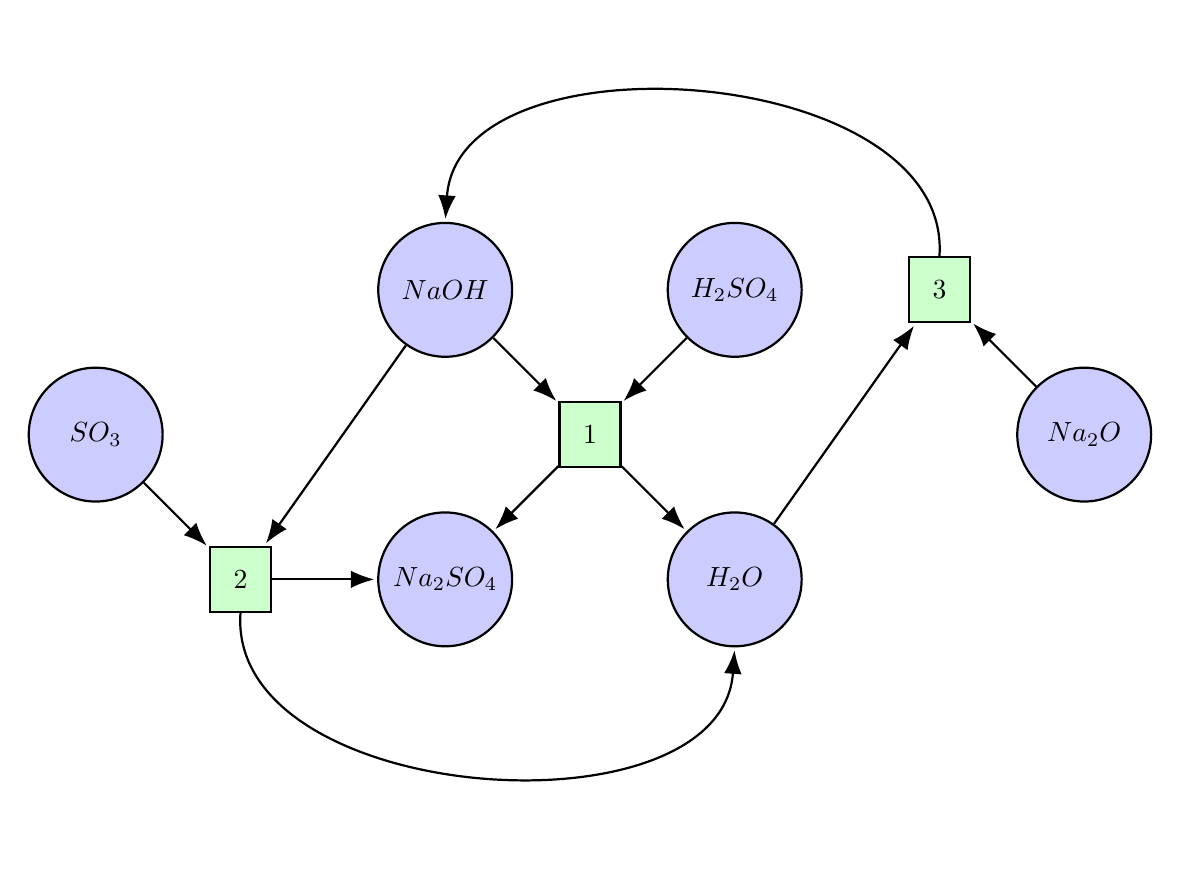
\begin{tikzpicture}[
    -{Latex[length=3mm]},
    shorten >=1pt,
    auto,
    node distance=2.6cm,
    thick,
    compound node/.style={circle,fill=blue!20,minimum width=1.7cm,draw},
    reaction node/.style={draw,thick,fill=green!20,inner sep=.3cm}]

  \node[compound node] (NaOH) {$NaOH$};
  \node[reaction node] (Reaction1) [below right of=NaOH] {$1$};
  \node[compound node] (H2SO4) [above right of=Reaction1] {$H_{2}SO_{4}$};
  \node[compound node] (Na2SO4) [below left of=Reaction1] {$Na_{2}SO_{4}$};
  \node[compound node] (H2O) [below right of=Reaction1] {$H_{2}O$};  
  \node[reaction node] (Reaction2) [left of=Na2SO4] {$2$};  
  \node[compound node] (SO3) [above left of=Reaction2] {$SO_{3}$};  
  \node[reaction node] (Reaction3) [right of=H2SO4] {$3$};  
  \node[compound node] (Na2O) [below right of=Reaction3] {$Na_{2}O$};  

  \path[every node/.style={font=\sffamily\small}]
    (NaOH) 
         edge node[left] {} (Reaction1)
         edge node[right] {} (Reaction2)
    (H2SO4) 
         edge node[right] {} (Reaction1)
    (Reaction1) 
         edge node [right] {} (Na2SO4)
         edge node [left] {} (H2O)
    (SO3) 
         edge node [left] {} (Reaction2)
    (Reaction2) 
         edge node [left] {} (Na2SO4)
         edge [bend right = 90] node [right] {} (H2O)
    (H2O) 
         edge node [left] {} (Reaction3)
    (Na2O) 
         edge node [right] {} (Reaction3)
    (Reaction3) 
         edge [bend right = 90] node [right] {} (NaOH);
\end{tikzpicture}

As far as each chemical compound must be of some of compound types -- this means, that each \emph{compound node from graph -- implicitly belongs to some compound type}. The same statement (about implicit correspondence to reaction type) is also true for \emph{reaction nodes}. In other words, each node of graph associated with \emph{discrete-valued random variable}: $X_i$, which corresponds either to compound type or reaction type: $x_i$. This can be represented using notation: $X_i = x_i$. 

For example, imagine node of graph, which corresponds to chemical compound $NaOH$, so, the possible affiliation of given compound node to type \lq \lq $Base$\rq \rq, might be denoted as: $X_{NaOH} = Base$.
\\

In general, we will use following notation for describing of probability of some specific configuration of node types of entire graph: $P(X_1 = x_1, X_2 = x_2, \cdots , X_n = x_n)$. In a little bit more succinct form: 
\begin{equation} \label{eq:probability_notation}
P(X_1 = x_1, X_2 = x_2, \cdots , X_n = x_n) = P(x_1, x_2, \cdots , x_n) = P(x)
\end{equation}

\section{Properties of chemical reactions graph}

Without loss of generalization -- we can state, that \emph{type of chemical compound depends only on types of reactions, in which given compound participates} (and vice versa -- type of chemical reaction depends only on types of compounds, which participate in given reaction). For illustration of this statement, lets consider following example: 
\\
\\
Having information -- that compound $X$ participates in reactions of following types:
\begin{enumerate}
    \item $Acidic\ Oxide + Basic\ Oxide \rightarrow Salt$
    \item $Basic\ Oxide + Water \rightarrow Base$
\end{enumerate}
We can easily \emph{infer} type of compound $X$: 
\begin{enumerate}
    \item For the first type of reaction: $Acidic\ Oxide + Basic\ Oxide \rightarrow Salt$ \\
             Set of possible compound types of $X$ is: $T_1 = \{Acidic\ Oxide, Basic\ Oxide, Salt\}$
    \item For the second type of reaction: $Basic\ Oxide + Water \rightarrow Base$ \\
             Set of possible compound types of $X$ is: $T_2 = \{Basic\ Oxide, Water, Base\}$
\end{enumerate}
So, the type of compound $X$ is $T_1 \cap T_2 = \{Basic\ Oxide\}$.
\\

\noindent Such property of graph of chemical reactions might be formalized as -- \emph{conditional independence of random variables of non-adjacent nodes}. This means, that graph of chemical reactions is actually can be treated as \emph{\textbf{Markov Random Field}} \cite{wikipedia_mrf}.
\\

Using result of Hammersley-Clifford Theorem, we can follow up, that probability distribution of configurations of graph -- can be factorized into positive functions defined on cliques that cover all the nodes and edges (also called a \emph{Gibbs distribution})\cite{hammersley_clifford_proof, wikipedia_hammersley_clifford}:

\begin{equation}
P(x) = {1 \over Z} \prod_{c \in C_G} \psi_{c}(x_c)
\end{equation}
where:
\begin{itemize} 
    \setlength \itemsep{0em}
    \item $Z$ -- normalization constant
    \item $x$ -- configuration of node types of entire graph, as described in equation \eqref{eq:probability_notation}
    \item $C_G$ -- set of all cliques of graph
    \item $x_c$ -- configuration of node types, which belongs to clique $c$
    \item $\psi_{c}$ --
\end{itemize}


\newpage

\begin{thebibliography}{9}

\bibitem{project_on_github}
  \url{https://github.com/lagodiuk/java-loopy-belief-propagation}.

\bibitem{fraud_detection}
  Leman Akoglu, Rishi Chandy, Christos Faloutsos,
  \emph{Opinion Fraud Detection in Online Reviews by Network Effects}.

\bibitem{understanding_bp}
  Jonathan S. Yedidia, William T. Freeman, and Yair Weiss,
  \emph{Understanding Belief Propagation and its Generalizations},
  TR2001-22, 
  November 2001.
  
\bibitem{wikipedia_mrf}
  \url{http://en.wikipedia.org/wiki/Markov_random_field#Definition}.
  
\bibitem{hammersley_clifford_proof}
  Samson Cheung,
  \emph{Proof of Hammersley-Clifford Theorem},
  \url{http://web.kaist.ac.kr/~kyomin/Fall09MRF/Hammersley-Clifford_Theorem.pdf},
  February 3, 2008.

\bibitem{wikipedia_hammersley_clifford}
  \url{http://en.wikipedia.org/wiki/Hammersley-Clifford_theorem}.

\end{thebibliography}

\end{document}